% Options for packages loaded elsewhere
\PassOptionsToPackage{unicode}{hyperref}
\PassOptionsToPackage{hyphens}{url}
%
\documentclass[
]{article}
\usepackage{amsmath,amssymb}
\usepackage{lmodern}
\usepackage{iftex}
\ifPDFTeX
  \usepackage[T1]{fontenc}
  \usepackage[utf8]{inputenc}
  \usepackage{textcomp} % provide euro and other symbols
\else % if luatex or xetex
  \usepackage{unicode-math}
  \defaultfontfeatures{Scale=MatchLowercase}
  \defaultfontfeatures[\rmfamily]{Ligatures=TeX,Scale=1}
\fi
% Use upquote if available, for straight quotes in verbatim environments
\IfFileExists{upquote.sty}{\usepackage{upquote}}{}
\IfFileExists{microtype.sty}{% use microtype if available
  \usepackage[]{microtype}
  \UseMicrotypeSet[protrusion]{basicmath} % disable protrusion for tt fonts
}{}
\makeatletter
\@ifundefined{KOMAClassName}{% if non-KOMA class
  \IfFileExists{parskip.sty}{%
    \usepackage{parskip}
  }{% else
    \setlength{\parindent}{0pt}
    \setlength{\parskip}{6pt plus 2pt minus 1pt}}
}{% if KOMA class
  \KOMAoptions{parskip=half}}
\makeatother
\usepackage{xcolor}
\usepackage[margin=1in]{geometry}
\usepackage{color}
\usepackage{fancyvrb}
\newcommand{\VerbBar}{|}
\newcommand{\VERB}{\Verb[commandchars=\\\{\}]}
\DefineVerbatimEnvironment{Highlighting}{Verbatim}{commandchars=\\\{\}}
% Add ',fontsize=\small' for more characters per line
\usepackage{framed}
\definecolor{shadecolor}{RGB}{248,248,248}
\newenvironment{Shaded}{\begin{snugshade}}{\end{snugshade}}
\newcommand{\AlertTok}[1]{\textcolor[rgb]{0.94,0.16,0.16}{#1}}
\newcommand{\AnnotationTok}[1]{\textcolor[rgb]{0.56,0.35,0.01}{\textbf{\textit{#1}}}}
\newcommand{\AttributeTok}[1]{\textcolor[rgb]{0.77,0.63,0.00}{#1}}
\newcommand{\BaseNTok}[1]{\textcolor[rgb]{0.00,0.00,0.81}{#1}}
\newcommand{\BuiltInTok}[1]{#1}
\newcommand{\CharTok}[1]{\textcolor[rgb]{0.31,0.60,0.02}{#1}}
\newcommand{\CommentTok}[1]{\textcolor[rgb]{0.56,0.35,0.01}{\textit{#1}}}
\newcommand{\CommentVarTok}[1]{\textcolor[rgb]{0.56,0.35,0.01}{\textbf{\textit{#1}}}}
\newcommand{\ConstantTok}[1]{\textcolor[rgb]{0.00,0.00,0.00}{#1}}
\newcommand{\ControlFlowTok}[1]{\textcolor[rgb]{0.13,0.29,0.53}{\textbf{#1}}}
\newcommand{\DataTypeTok}[1]{\textcolor[rgb]{0.13,0.29,0.53}{#1}}
\newcommand{\DecValTok}[1]{\textcolor[rgb]{0.00,0.00,0.81}{#1}}
\newcommand{\DocumentationTok}[1]{\textcolor[rgb]{0.56,0.35,0.01}{\textbf{\textit{#1}}}}
\newcommand{\ErrorTok}[1]{\textcolor[rgb]{0.64,0.00,0.00}{\textbf{#1}}}
\newcommand{\ExtensionTok}[1]{#1}
\newcommand{\FloatTok}[1]{\textcolor[rgb]{0.00,0.00,0.81}{#1}}
\newcommand{\FunctionTok}[1]{\textcolor[rgb]{0.00,0.00,0.00}{#1}}
\newcommand{\ImportTok}[1]{#1}
\newcommand{\InformationTok}[1]{\textcolor[rgb]{0.56,0.35,0.01}{\textbf{\textit{#1}}}}
\newcommand{\KeywordTok}[1]{\textcolor[rgb]{0.13,0.29,0.53}{\textbf{#1}}}
\newcommand{\NormalTok}[1]{#1}
\newcommand{\OperatorTok}[1]{\textcolor[rgb]{0.81,0.36,0.00}{\textbf{#1}}}
\newcommand{\OtherTok}[1]{\textcolor[rgb]{0.56,0.35,0.01}{#1}}
\newcommand{\PreprocessorTok}[1]{\textcolor[rgb]{0.56,0.35,0.01}{\textit{#1}}}
\newcommand{\RegionMarkerTok}[1]{#1}
\newcommand{\SpecialCharTok}[1]{\textcolor[rgb]{0.00,0.00,0.00}{#1}}
\newcommand{\SpecialStringTok}[1]{\textcolor[rgb]{0.31,0.60,0.02}{#1}}
\newcommand{\StringTok}[1]{\textcolor[rgb]{0.31,0.60,0.02}{#1}}
\newcommand{\VariableTok}[1]{\textcolor[rgb]{0.00,0.00,0.00}{#1}}
\newcommand{\VerbatimStringTok}[1]{\textcolor[rgb]{0.31,0.60,0.02}{#1}}
\newcommand{\WarningTok}[1]{\textcolor[rgb]{0.56,0.35,0.01}{\textbf{\textit{#1}}}}
\usepackage{graphicx}
\makeatletter
\def\maxwidth{\ifdim\Gin@nat@width>\linewidth\linewidth\else\Gin@nat@width\fi}
\def\maxheight{\ifdim\Gin@nat@height>\textheight\textheight\else\Gin@nat@height\fi}
\makeatother
% Scale images if necessary, so that they will not overflow the page
% margins by default, and it is still possible to overwrite the defaults
% using explicit options in \includegraphics[width, height, ...]{}
\setkeys{Gin}{width=\maxwidth,height=\maxheight,keepaspectratio}
% Set default figure placement to htbp
\makeatletter
\def\fps@figure{htbp}
\makeatother
\setlength{\emergencystretch}{3em} % prevent overfull lines
\providecommand{\tightlist}{%
  \setlength{\itemsep}{0pt}\setlength{\parskip}{0pt}}
\setcounter{secnumdepth}{-\maxdimen} % remove section numbering
\ifLuaTeX
  \usepackage{selnolig}  % disable illegal ligatures
\fi
\IfFileExists{bookmark.sty}{\usepackage{bookmark}}{\usepackage{hyperref}}
\IfFileExists{xurl.sty}{\usepackage{xurl}}{} % add URL line breaks if available
\urlstyle{same} % disable monospaced font for URLs
\hypersetup{
  hidelinks,
  pdfcreator={LaTeX via pandoc}}

\author{}
\date{\vspace{-2.5em}}

\begin{document}

\begin{center}\rule{0.5\linewidth}{0.5pt}\end{center}

\#output: rmarkdown::github\_document output: pdf\_document: default
html\_document: default editor\_options: markdown: wrap: 72 ---

\hypertarget{visstatistics}{%
\section{visStatistics}\label{visstatistics}}

Visualization of the statistical hypothesis test between two groups of
categorical or numerical data.

Statistical consulting requires often both a quick first visualization
and a reproducible statistical analysis of the presented raw data. The
package \texttt{visStatistics} with its core function \texttt{visstat()}
fulfils this need. Based on a decision tree it picks the statistical
hypothesis test with the highest statistical power between the dependent
variable (response) \texttt{varsample} and the independent variable
(feature) \texttt{varfactor}. The corresponding test statistics
including eventual post-hoc-analysis are returned and a graph showing
key statistics of the underlying test is generated.

This fully automated workflow is especially suited for browser based
interfaces to server-based deployments of R and has been successfully
implemented to analyse medical raw data in an unbiased fashion.

A detailed description of the package's functionality and its underlying
decision tree, can be found in the \texttt{vignette} accompanying this
package.

\hypertarget{implemented-tests}{%
\subsection{Implemented tests}\label{implemented-tests}}

\texttt{lm()}, \texttt{t.test()}, \texttt{wilcox.test()},
\texttt{aov()}, \texttt{kruskal.test()}, \texttt{fisher.test()},
\texttt{chisqu.test()}

\hypertarget{implemented-tests-to-check-the-normal-distribution-of-standardized-residuals}{%
\subsubsection{Implemented tests to check the normal distribution of
standardized
residuals}\label{implemented-tests-to-check-the-normal-distribution-of-standardized-residuals}}

\texttt{shapiro.test()} and \texttt{ad.test()}

\hypertarget{implemented-post-hoc-tests}{%
\subsubsection{Implemented post-hoc
tests}\label{implemented-post-hoc-tests}}

\texttt{TukeyHSD()} for \texttt{aov()}and
\texttt{pairwise.wilcox.test()} for \texttt{kruskal.test()}

\hypertarget{installation-from-cran}{%
\subsection{Installation from CRAN}\label{installation-from-cran}}

\begin{enumerate}
\def\labelenumi{\arabic{enumi}.}
\tightlist
\item
  Install the package \texttt{install.packages("visStatistics")}
\item
  Load the package \texttt{library(visStatistics)}
\end{enumerate}

\hypertarget{installation-from-github-always-latest-developing-version}{%
\subsection{Installation from GitHub (always latest, developing
version)}\label{installation-from-github-always-latest-developing-version}}

\begin{enumerate}
\def\labelenumi{\arabic{enumi}.}
\tightlist
\item
  Install the devtools package from CRAN. Invoke R and type
  \texttt{install.packages("devtools")}
\item
  Load the devtools package. \texttt{library(devtools)}
\item
  Install the package from the github-repository
  \texttt{install\_github("shhschilling/visStatistics")}
\item
  Load the package \texttt{library(visStatistics)}
\item
  Help on the function usage \texttt{?visstat}
\end{enumerate}

\hypertarget{getting-started}{%
\subsection{Getting Started}\label{getting-started}}

The package vignette allows you to get familiar with all features of
\texttt{visStatistics}. It documents in detail the algorithm of the
decision tree illustrated by examples.

\hypertarget{examples}{%
\subsection{Examples}\label{examples}}

\begin{Shaded}
\begin{Highlighting}[]
\FunctionTok{library}\NormalTok{(visStatistics)}
\end{Highlighting}
\end{Shaded}

\hypertarget{welch-two-sample-t.test}{%
\subsubsection{Welch Two Sample t.test}\label{welch-two-sample-t.test}}

\hypertarget{insectsprays-data-set}{%
\paragraph{InsectSprays data set}\label{insectsprays-data-set}}

\begin{Shaded}
\begin{Highlighting}[]
\NormalTok{InsectSpraysAB }\OtherTok{\textless{}{-}}\NormalTok{ InsectSprays[}\FunctionTok{which}\NormalTok{(InsectSprays}\SpecialCharTok{$}\NormalTok{spray }\SpecialCharTok{==} \StringTok{"A"} \SpecialCharTok{|}\NormalTok{ InsectSprays}\SpecialCharTok{$}\NormalTok{spray }\SpecialCharTok{==} \StringTok{"B"}\NormalTok{), ]}
\NormalTok{InsectSpraysAB}\SpecialCharTok{$}\NormalTok{spray }\OtherTok{\textless{}{-}} \FunctionTok{factor}\NormalTok{(InsectSpraysAB}\SpecialCharTok{$}\NormalTok{spray)}
\FunctionTok{visstat}\NormalTok{(InsectSpraysAB, }\StringTok{"count"}\NormalTok{, }\StringTok{"spray"}\NormalTok{)}
\CommentTok{\#\textgreater{} Warning in mtext(two\_sample\_title): conversion failure on \textquotesingle{}Welch Two Sample}
\CommentTok{\#\textgreater{} t{-}test, α = 0.05\textquotesingle{} in \textquotesingle{}mbcsToSbcs\textquotesingle{}: dot substituted for \textless{}ce\textgreater{}}
\CommentTok{\#\textgreater{} Warning in mtext(two\_sample\_title): conversion failure on \textquotesingle{}Welch Two Sample}
\CommentTok{\#\textgreater{} t{-}test, α = 0.05\textquotesingle{} in \textquotesingle{}mbcsToSbcs\textquotesingle{}: dot substituted for \textless{}b1\textgreater{}}
\CommentTok{\#\textgreater{} Warning in mtext(two\_sample\_title): conversion failure on \textquotesingle{} p = 0.65, p \textgreater{} α\textquotesingle{} in}
\CommentTok{\#\textgreater{} \textquotesingle{}mbcsToSbcs\textquotesingle{}: dot substituted for \textless{}ce\textgreater{}}
\CommentTok{\#\textgreater{} Warning in mtext(two\_sample\_title): conversion failure on \textquotesingle{} p = 0.65, p \textgreater{} α\textquotesingle{} in}
\CommentTok{\#\textgreater{} \textquotesingle{}mbcsToSbcs\textquotesingle{}: dot substituted for \textless{}b1\textgreater{}}
\end{Highlighting}
\end{Shaded}

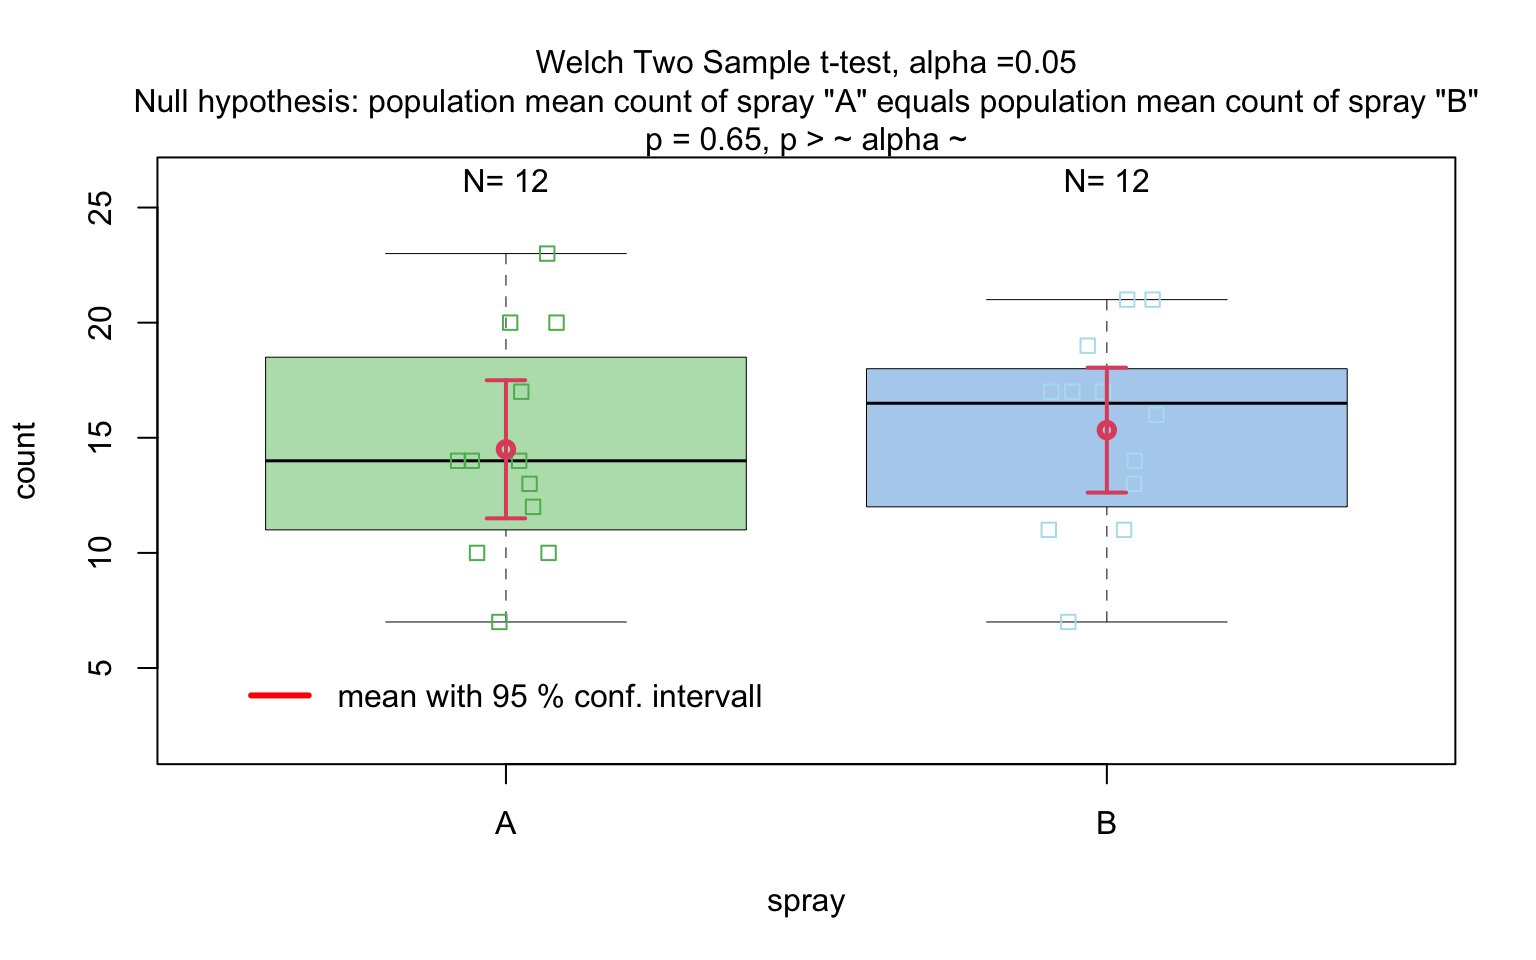
\includegraphics[width=1\linewidth]{man/figures/README-unnamed-chunk-2-1}

\hypertarget{mtcars-data-set}{%
\paragraph{mtcars data set}\label{mtcars-data-set}}

\begin{Shaded}
\begin{Highlighting}[]
\NormalTok{mtcars}\SpecialCharTok{$}\NormalTok{am }\OtherTok{\textless{}{-}} \FunctionTok{as.factor}\NormalTok{(mtcars}\SpecialCharTok{$}\NormalTok{am)}
\NormalTok{ttestStatistics }\OtherTok{\textless{}{-}} \FunctionTok{visstat}\NormalTok{(mtcars, }\StringTok{"mpg"}\NormalTok{, }\StringTok{"am"}\NormalTok{)}
\CommentTok{\#\textgreater{} Warning in mtext(two\_sample\_title): conversion failure on \textquotesingle{}Welch Two Sample}
\CommentTok{\#\textgreater{} t{-}test, α = 0.05\textquotesingle{} in \textquotesingle{}mbcsToSbcs\textquotesingle{}: dot substituted for \textless{}ce\textgreater{}}
\CommentTok{\#\textgreater{} Warning in mtext(two\_sample\_title): conversion failure on \textquotesingle{}Welch Two Sample}
\CommentTok{\#\textgreater{} t{-}test, α = 0.05\textquotesingle{} in \textquotesingle{}mbcsToSbcs\textquotesingle{}: dot substituted for \textless{}b1\textgreater{}}
\CommentTok{\#\textgreater{} Warning in mtext(two\_sample\_title): conversion failure on \textquotesingle{} p = 0.0014, p \textless{} α\textquotesingle{}}
\CommentTok{\#\textgreater{} in \textquotesingle{}mbcsToSbcs\textquotesingle{}: dot substituted for \textless{}ce\textgreater{}}
\CommentTok{\#\textgreater{} Warning in mtext(two\_sample\_title): conversion failure on \textquotesingle{} p = 0.0014, p \textless{} α\textquotesingle{}}
\CommentTok{\#\textgreater{} in \textquotesingle{}mbcsToSbcs\textquotesingle{}: dot substituted for \textless{}b1\textgreater{}}
\end{Highlighting}
\end{Shaded}

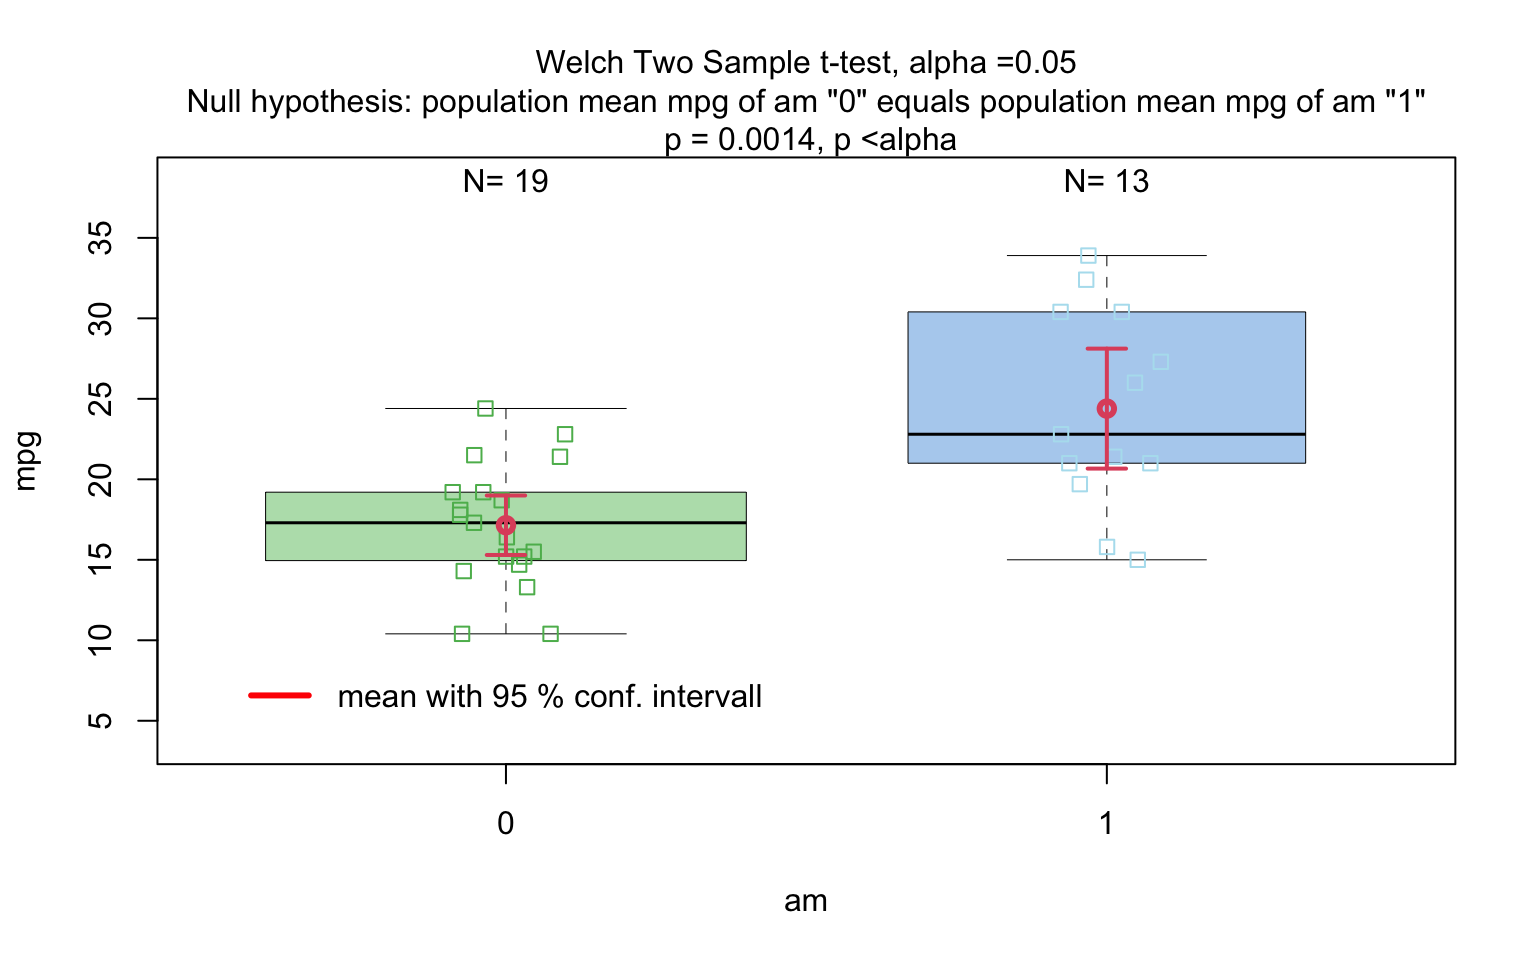
\includegraphics[width=1\linewidth]{man/figures/README-unnamed-chunk-4-1}

Uncomment below line to print out summary statistics:

\begin{Shaded}
\begin{Highlighting}[]
\CommentTok{\# ttestStatistics}
\end{Highlighting}
\end{Shaded}

\hypertarget{wilcoxon-rank-sum-test-with-continuity-correction}{%
\subsubsection{Wilcoxon rank sum test with continuity
correction}\label{wilcoxon-rank-sum-test-with-continuity-correction}}

\begin{Shaded}
\begin{Highlighting}[]
\FunctionTok{visstat}\NormalTok{(ToothGrowth, }\StringTok{"len"}\NormalTok{, }\StringTok{"supp"}\NormalTok{)}
\CommentTok{\#\textgreater{} Warning in wilcox.test.default(x = DATA[[1L]], y = DATA[[2L]], ...): cannot}
\CommentTok{\#\textgreater{} compute exact p{-}value with ties}
\CommentTok{\#\textgreater{} Warning in mtext(two\_sample\_title): conversion failure on \textquotesingle{}Wilcoxon rank sum}
\CommentTok{\#\textgreater{} test with continuity correction, α = 0.05\textquotesingle{} in \textquotesingle{}mbcsToSbcs\textquotesingle{}: dot substituted for}
\CommentTok{\#\textgreater{} \textless{}ce\textgreater{}}
\CommentTok{\#\textgreater{} Warning in mtext(two\_sample\_title): conversion failure on \textquotesingle{}Wilcoxon rank sum}
\CommentTok{\#\textgreater{} test with continuity correction, α = 0.05\textquotesingle{} in \textquotesingle{}mbcsToSbcs\textquotesingle{}: dot substituted for}
\CommentTok{\#\textgreater{} \textless{}b1\textgreater{}}
\CommentTok{\#\textgreater{} Warning in mtext(two\_sample\_title): conversion failure on \textquotesingle{} p = 0.064, p \textgreater{} α\textquotesingle{}}
\CommentTok{\#\textgreater{} in \textquotesingle{}mbcsToSbcs\textquotesingle{}: dot substituted for \textless{}ce\textgreater{}}
\CommentTok{\#\textgreater{} Warning in mtext(two\_sample\_title): conversion failure on \textquotesingle{} p = 0.064, p \textgreater{} α\textquotesingle{}}
\CommentTok{\#\textgreater{} in \textquotesingle{}mbcsToSbcs\textquotesingle{}: dot substituted for \textless{}b1\textgreater{}}
\end{Highlighting}
\end{Shaded}

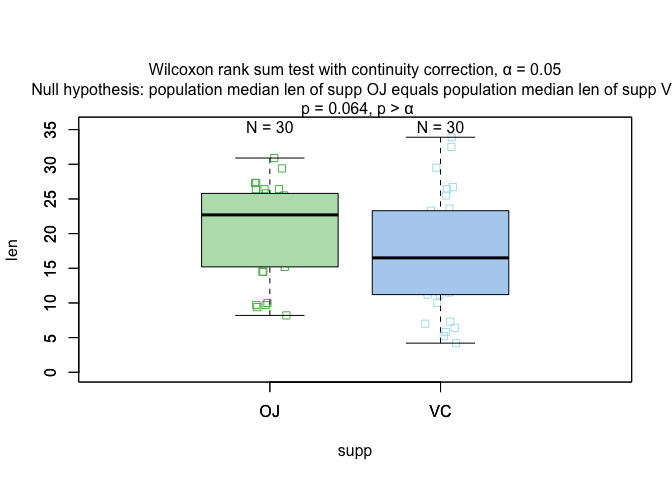
\includegraphics[width=1\linewidth]{man/figures/README-unnamed-chunk-6-1}

\hypertarget{one-way-test}{%
\subsubsection{One-way test}\label{one-way-test}}

\begin{Shaded}
\begin{Highlighting}[]
\NormalTok{anova\_npk }\OtherTok{\textless{}{-}} \FunctionTok{visstat}\NormalTok{(npk, }\StringTok{"yield"}\NormalTok{, }\StringTok{"block"}\NormalTok{)}
\end{Highlighting}
\end{Shaded}

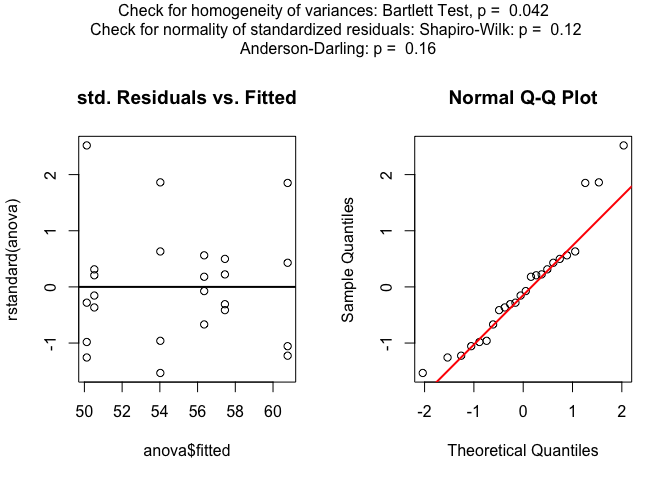
\includegraphics[width=1\linewidth]{man/figures/README-unnamed-chunk-7-1}
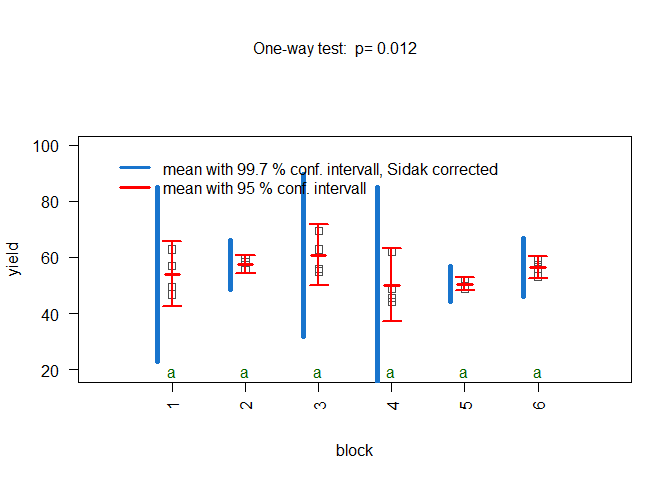
\includegraphics[width=1\linewidth]{man/figures/README-unnamed-chunk-7-2}

\hypertarget{kruskal-wallis-test}{%
\subsubsection{Kruskal-Wallis test}\label{kruskal-wallis-test}}

The generated graphs can be saved in all available formats of the
\texttt{Cairo} package. Here we save the graphical output of type
``pdf'' in the \texttt{plotDirectory} \texttt{tempdir()}:

\begin{Shaded}
\begin{Highlighting}[]
\FunctionTok{visstat}\NormalTok{(iris, }\StringTok{"Petal.Width"}\NormalTok{, }\StringTok{"Species"}\NormalTok{, }\AttributeTok{graphicsoutput =} \StringTok{"pdf"}\NormalTok{, }\AttributeTok{plotDirectory =} \FunctionTok{tempdir}\NormalTok{())}
\end{Highlighting}
\end{Shaded}

\hypertarget{linear-regression}{%
\subsubsection{Linear Regression}\label{linear-regression}}

\begin{Shaded}
\begin{Highlighting}[]
\NormalTok{linreg\_cars }\OtherTok{\textless{}{-}} \FunctionTok{visstat}\NormalTok{(cars, }\StringTok{"dist"}\NormalTok{, }\StringTok{"speed"}\NormalTok{)}
\end{Highlighting}
\end{Shaded}

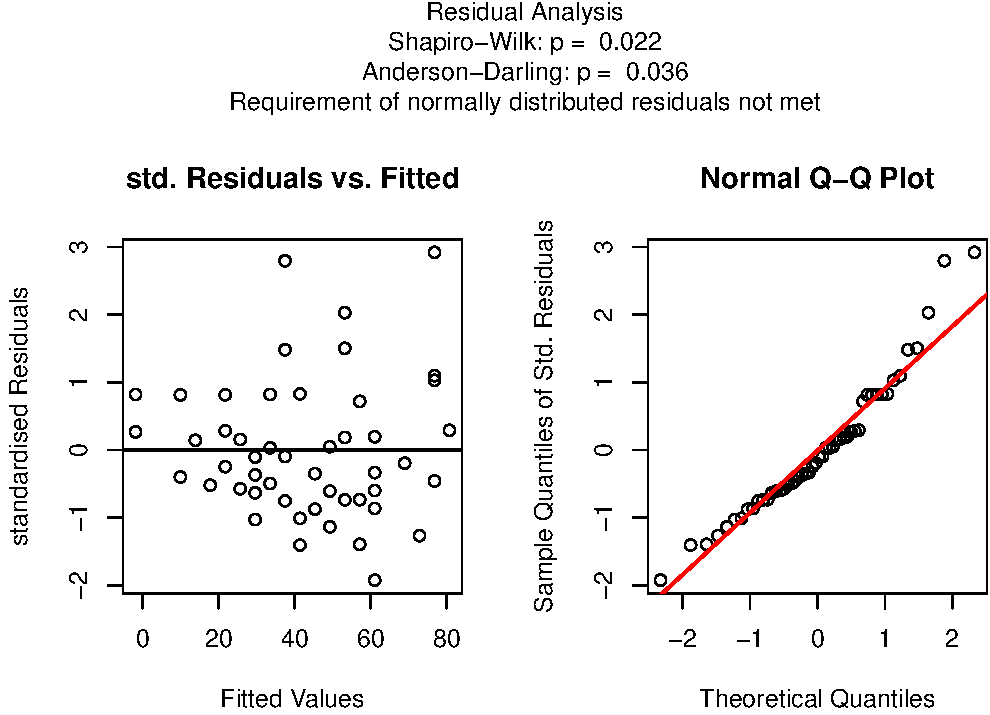
\includegraphics[width=1\linewidth]{man/figures/README-unnamed-chunk-9-1}
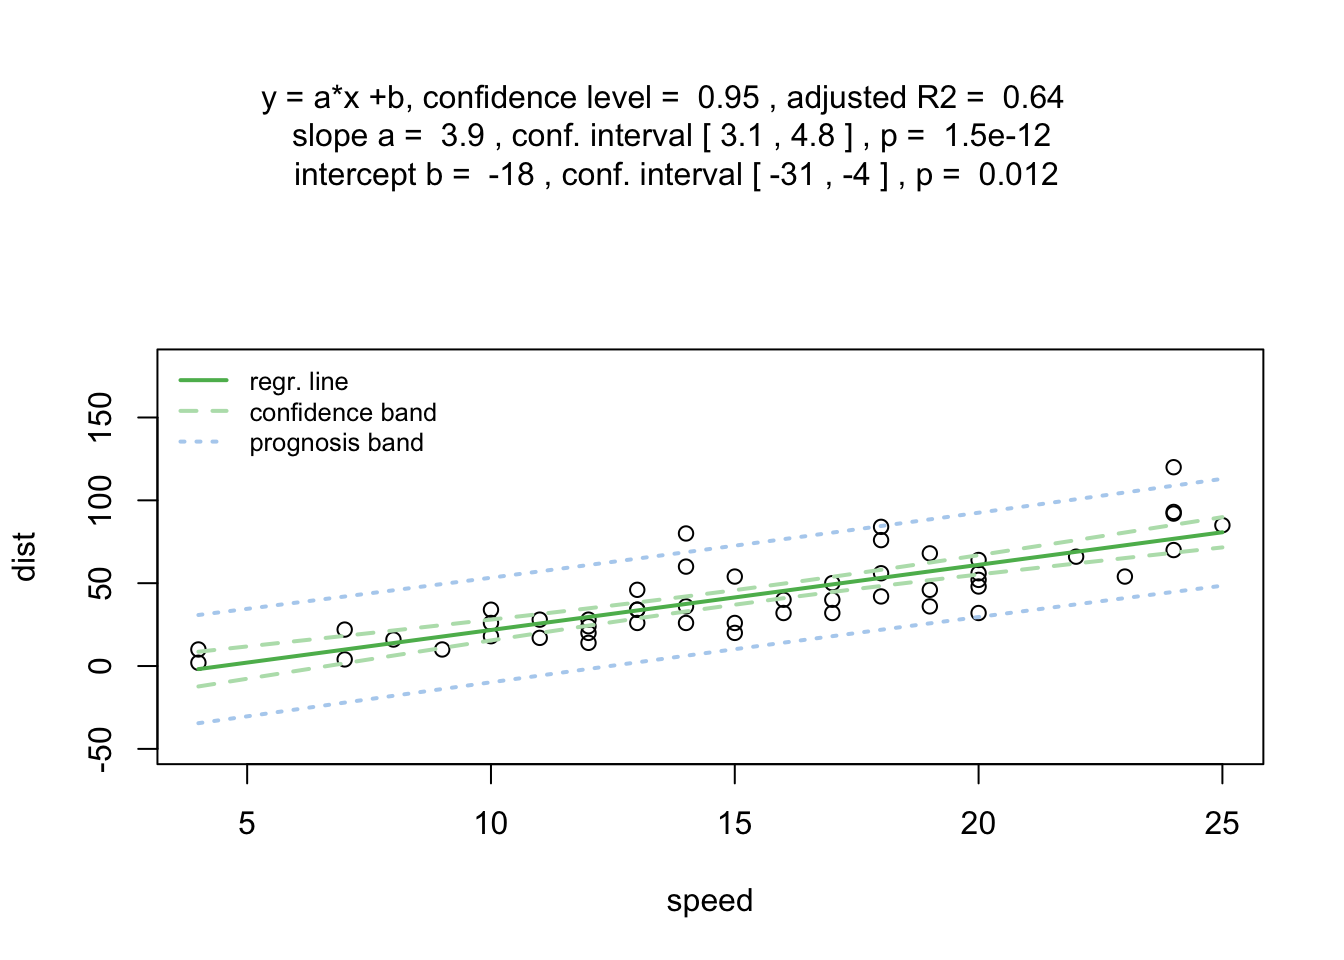
\includegraphics[width=1\linewidth]{man/figures/README-unnamed-chunk-9-2}

Increasing the confidence level \texttt{conf.level} from the default
0.95 to 0.99 leads two wider confidence and prediction bands:

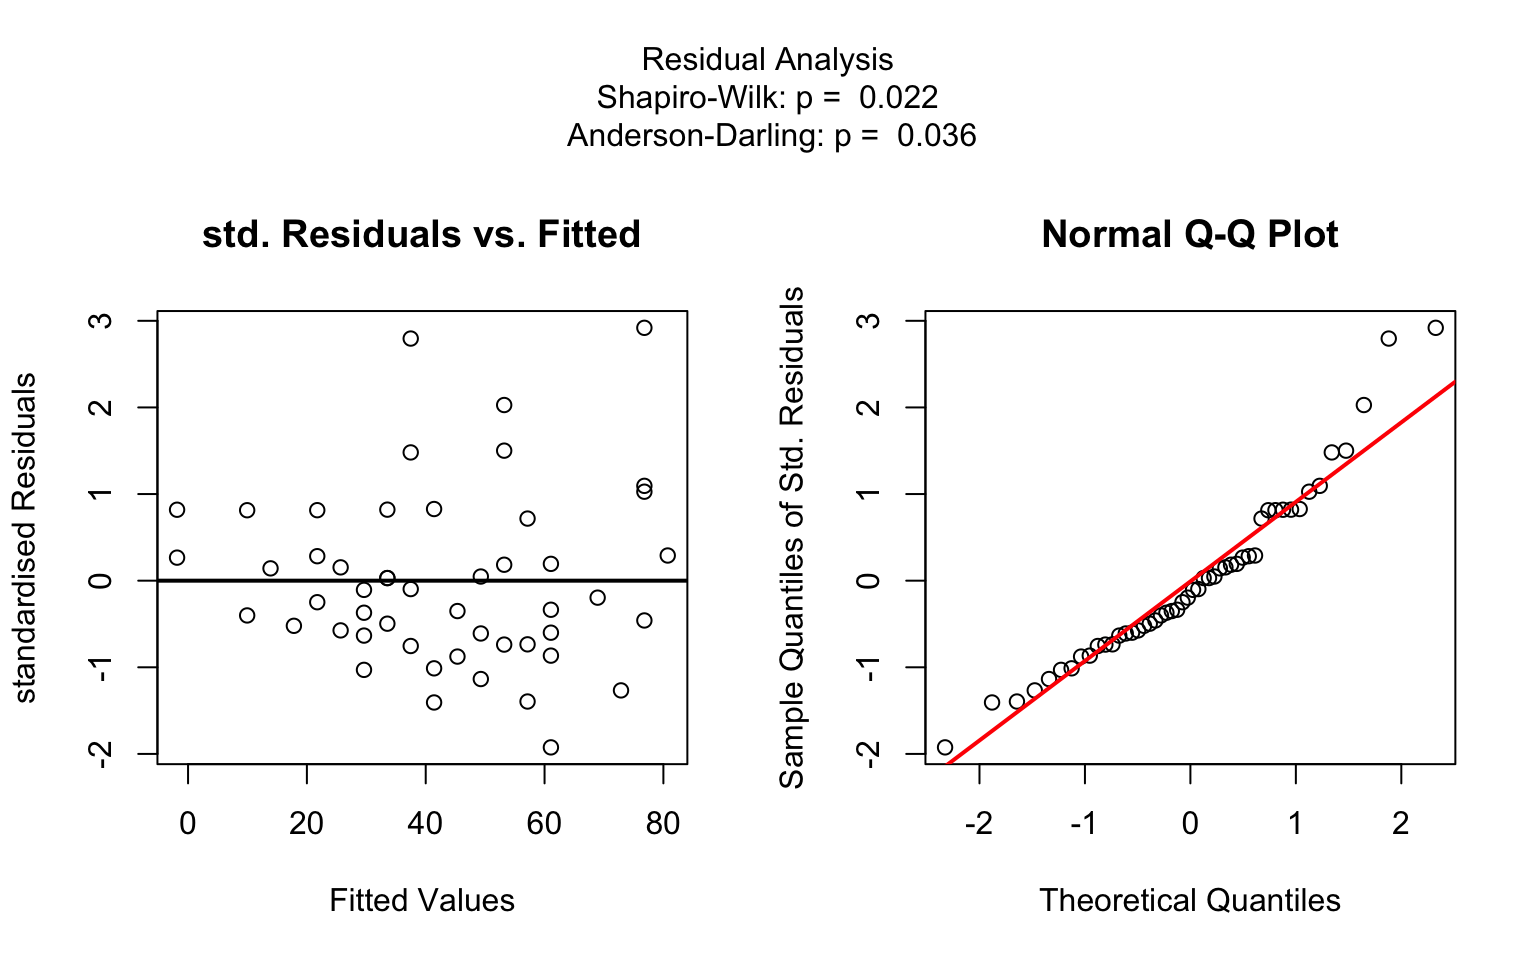
\includegraphics[width=1\linewidth]{man/figures/README-pressure-1}
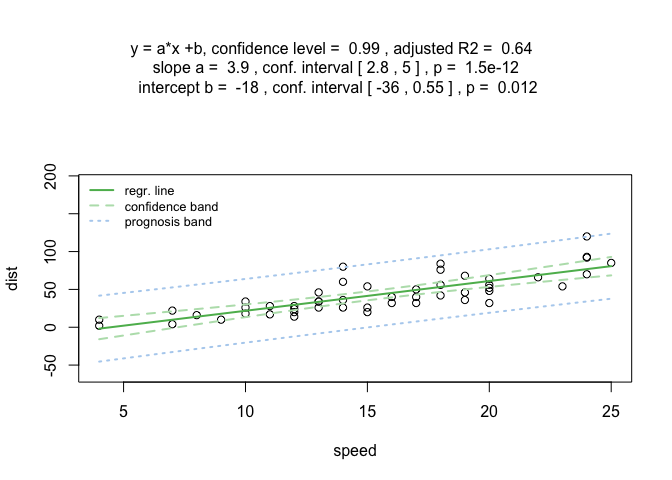
\includegraphics[width=1\linewidth]{man/figures/README-pressure-2}

\hypertarget{pearsons-chi-squared-test}{%
\subsubsection{Pearson's Chi-squared
test}\label{pearsons-chi-squared-test}}

Count data sets are often presented as multidimensional arrays,
so-called contingency tables, whereas \texttt{visstat()} requires a
\texttt{data.frame} with a column structure. Arrays can be transformed
to this column wise structure with the helper function
\texttt{counts\_to\_cases()}:

\begin{Shaded}
\begin{Highlighting}[]
\NormalTok{HairEyeColorDataFrame }\OtherTok{\textless{}{-}} \FunctionTok{counts\_to\_cases}\NormalTok{(}\FunctionTok{as.data.frame}\NormalTok{(HairEyeColor))}
\FunctionTok{visstat}\NormalTok{(HairEyeColorDataFrame, }\StringTok{"Hair"}\NormalTok{, }\StringTok{"Eye"}\NormalTok{)}
\end{Highlighting}
\end{Shaded}

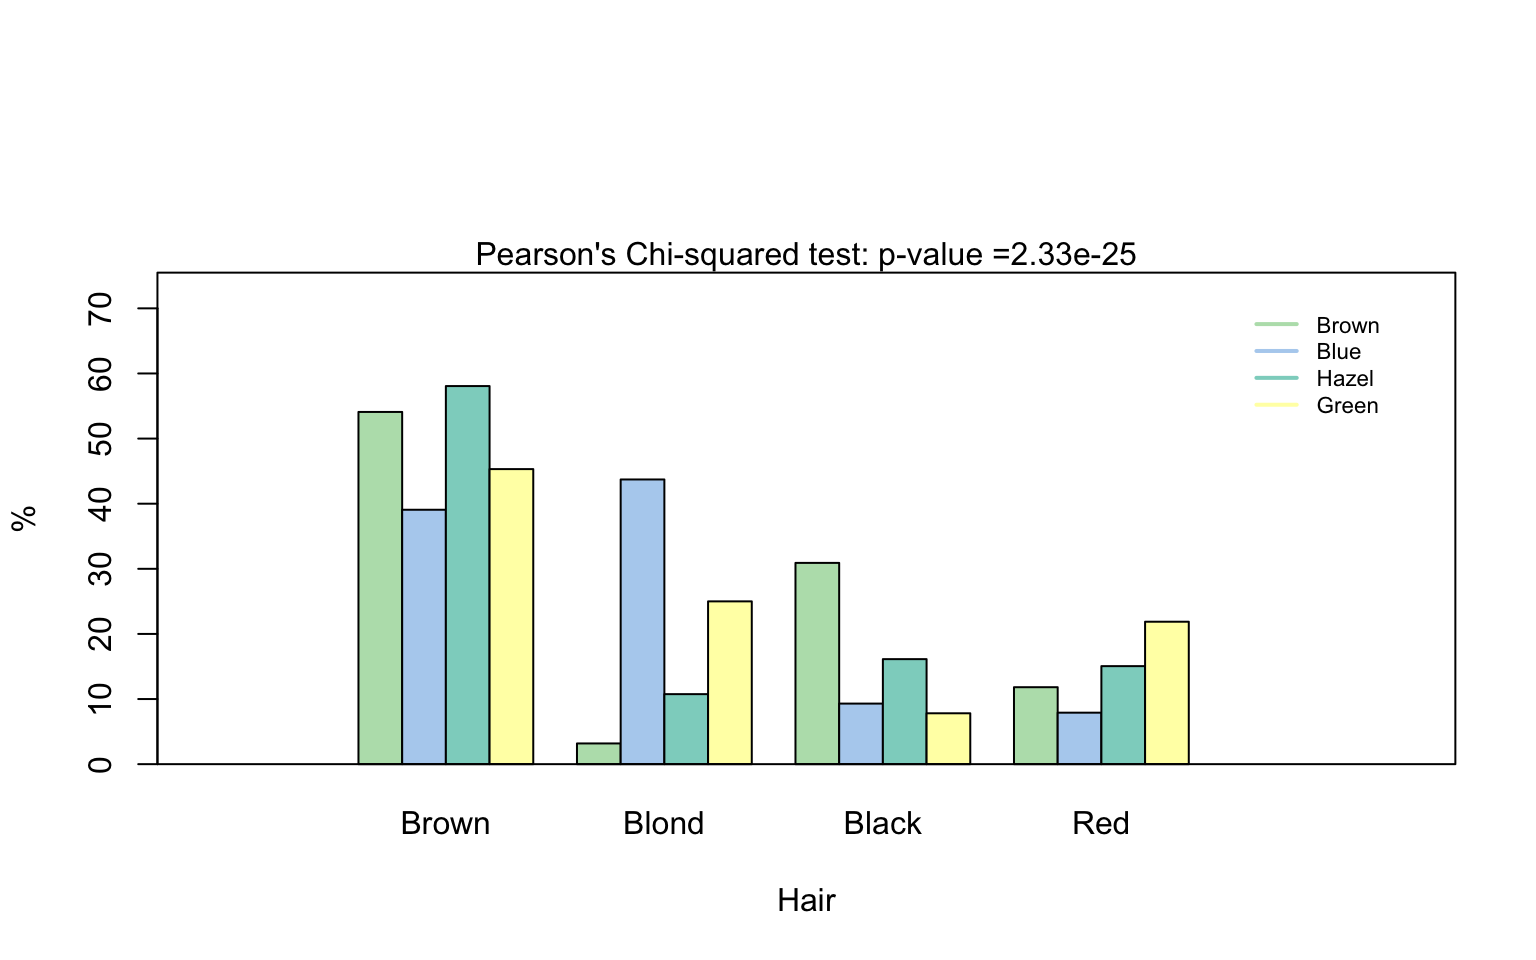
\includegraphics[width=1\linewidth]{man/figures/README-unnamed-chunk-10-1}
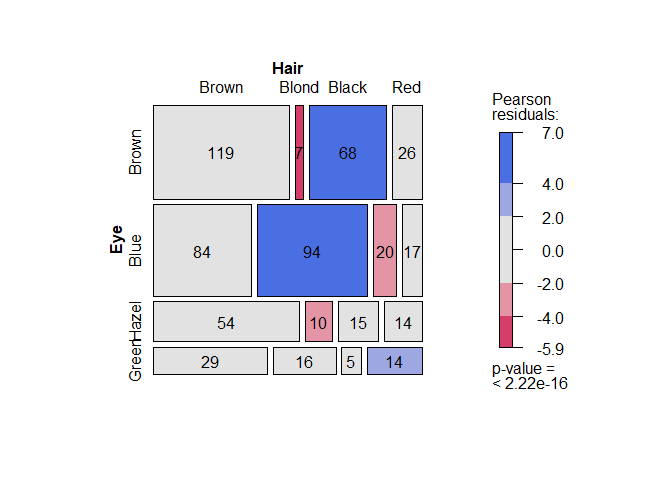
\includegraphics[width=1\linewidth]{man/figures/README-unnamed-chunk-10-2}

\hypertarget{fishers-exact-test}{%
\subsubsection{Fisher's exact test}\label{fishers-exact-test}}

\begin{Shaded}
\begin{Highlighting}[]
\NormalTok{HairEyeColorMaleFisher }\OtherTok{\textless{}{-}}\NormalTok{ HairEyeColor[, , }\DecValTok{1}\NormalTok{]}
\CommentTok{\# slicing out a 2 x2 contingency table}
\NormalTok{blackBrownHazelGreen }\OtherTok{\textless{}{-}}\NormalTok{ HairEyeColorMaleFisher[}\DecValTok{1}\SpecialCharTok{:}\DecValTok{2}\NormalTok{, }\DecValTok{3}\SpecialCharTok{:}\DecValTok{4}\NormalTok{]}
\NormalTok{blackBrownHazelGreen }\OtherTok{\textless{}{-}} \FunctionTok{counts\_to\_cases}\NormalTok{(}\FunctionTok{as.data.frame}\NormalTok{(blackBrownHazelGreen))}
\NormalTok{fisher\_stats }\OtherTok{\textless{}{-}} \FunctionTok{visstat}\NormalTok{(blackBrownHazelGreen, }\StringTok{"Hair"}\NormalTok{, }\StringTok{"Eye"}\NormalTok{)}
\end{Highlighting}
\end{Shaded}

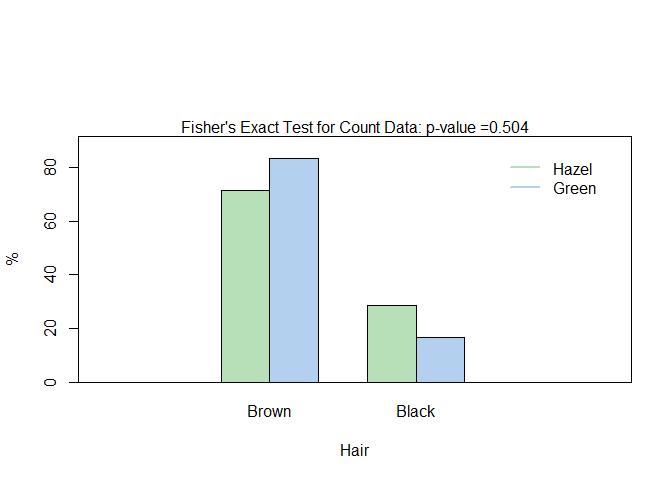
\includegraphics[width=1\linewidth]{man/figures/README-unnamed-chunk-11-1}
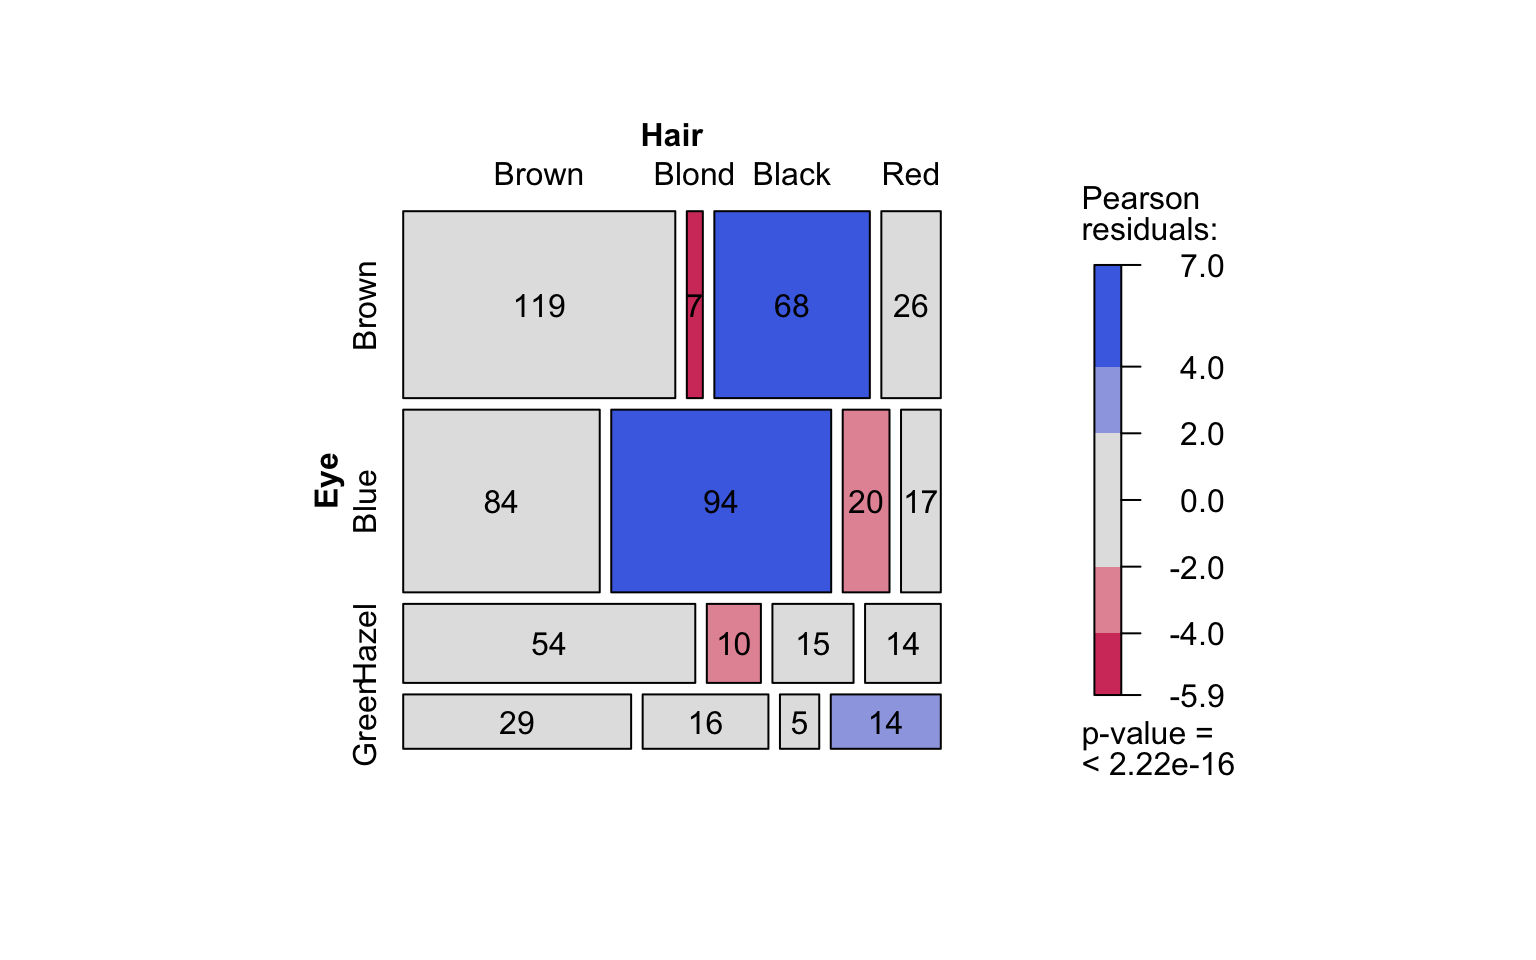
\includegraphics[width=1\linewidth]{man/figures/README-unnamed-chunk-11-2}

For details regarding the generated mosaic plots, please refer to the
\texttt{mosaic()} in the \texttt{vcd} package.

\end{document}
